\chapter{Générez et exportez vos clés GPG}

Let's go ! Vous allez faire votre première action concrète pour
l'utilisation de GPG : générer votre première clé !\\Ou plus exactement
votre première paire de clés, puisque rappelez vous : chaque clé GPG a
en fait une face privée et une face publique.

\textbf{Cet article peut sembler long ou ardu, mais il est important.
Créer les clés prend juste quelques minutes et vous n'avez quasiment
rien à faire. Donc s'il vous plait, prenez votre temps.}

\begin{notice}
S'il y a des gens inquiets: vous pouvez tout à fait utiliser une adresse
bidon pour ce tutoriel. Après tout, c'est bien ce que je fais avec
l'adresse du tuto.

Après cela, vous vous refaîtes des clés gpg avec votre vraie adresse, en
suivant à nouveau le tutoriel, mais vous ne les envoyez pas ici. Pas de
soucis !
\end{notice}

\section{Génération de la clé}\label{guxe9nuxe9ration-de-la-cluxe9}

Ouvrez votre gestionnaire de clés : Kgpg, Kleopatra ou Énigmail (ou un
autre encore\ldots{}) et chercher l'option de création de clés.

Sous Kleopatra, il s'agit de \textbf{\emph{Fichier \textgreater{}
Nouveau certificat \textgreater{} Créer une paire de clés personnelles
OpenPGP}}.

Sous Kgpg, il s'agit de \textbf{\emph{Clés \textgreater{} Générer une
paire de clés}}.

Sous Énigmail (donc dans Thunderbird lui-même), il s'agit de
\textbf{\emph{OpenPGP \textgreater{} Gestion de clés}}. Sélectionnez
alors \textbf{\emph{Générer \textgreater{} Nouvelle paire de clés.}}

\subsubsection{L'adresse à indiquer}\label{ladresse-uxe0-indiquer}

Le logiciel vous demandera quelle(s) adresse(s) vous voulez sécuriser
avec votre clé. Vous pouvez en effet mettre plusieurs adresses. Pour le
moment, c'est mieux de n'en mettre qu'une.

\subsubsection{Algorithme}\label{algorithme}

Il vous sera peut-être proposé plusieurs algorithmes : DSA \& ElGamal,
RSA \& RSA ou RSA.

Choisissez RSA \& RSA (dans Enigmail, onglet \emph{Avancé\ldots{}}, il
s'agit de l'option RSA). Il s'agit de la combinaison d'algorithmes la
plus forte et permet de chiffrer et signer.

\subsubsection{Longueur de clé}\label{longueur-de-cluxe9}

On vous demandera aussi la longueur de la clé à générer, avec ce choix :
1024, 2048 ou 4096 bits. Il y a peut-être d'autres choix, mais
globalement c'est ça.

Cette question indique en fait quelle sera la force de votre clé, sa
solidité, mais aussi le temps necessaire à la génération de la clé.

La longueur de clé choisie va demander au \emph{générateur de hasard} de
votre ordinateur une certaine quantité d'\emph{entropie}, quantité
exprimée avec ce nombre en \emph{bits}.

\begin{notice}
Je dois ici avouer ne pas comprendre vraiment le fondement profond de la
chose.\\Dès que j'essaye de comprendre ces concepts d'entropie, de
quantité d'entropie, je suis largué.\\En revanche, ce que je comprends
bien, c'est que plus il y a d'entropie, plus la clé est forte et le
chiffrement difficile à casser.
\end{notice}

Aujourd'hui, il est très recommandé de mettre 4096 bits. D'ailleurs je
pense que les prochaines versions des logiciels OpenPGP verront
apparaître des tailles de clés supérieures (puisque pour l'instant, 4096
est la limite) et/ou de nouveaux algorithmes.

La génération de la clé va prendre pas mal de temps. Il ne faut donc pas
s'inquiéter ou arreter votre logiciel précipitement.

Vous pouvez réduire ce temps en utilisant votre ordinateur. En effet,
plus vous utilisez votre ordinateur (particulièrement les accès
disques), plus vous générez l'entropie pour le générateur de
hasard.\\L'idéal, c'est donc d'en profiter pour mettre à jour sa
distribution (haute utilisation du disque dur) et d'aller jeter un coup
d'oeil sur la dernière vidéo de chaton sur vimeo\ldots{}

\subsubsection{Durée de validité}\label{duruxe9e-de-validituxe9}

On vous demandera normalement combien de temps la clé doit rester
valide.

Moi, ce que je fais, c'est que je donne une durée de validité d'un an,
que je repousse juste avant (un mois avant) l'échéance.\\Il s'agit ici
de ce qu'on appellerait un \emph{dispositif de l'homme mort} : si vous
veniez à perdre le contrôle de votre clé, celle-ci s'\emph{éteindra}
d'elle-même.

\subsubsection{Passphrase}\label{passphrase}

Il vous sera demandé une \textbf{\emph{passphrase}}. Une
\emph{passphrase} est un mot de passe très long. Donc par exemple quinze
ou vingt caractères.

Il existe plusieurs excellentes méthodes pour créer un bon mot de passe.

\begin{figure}[h]
\centering
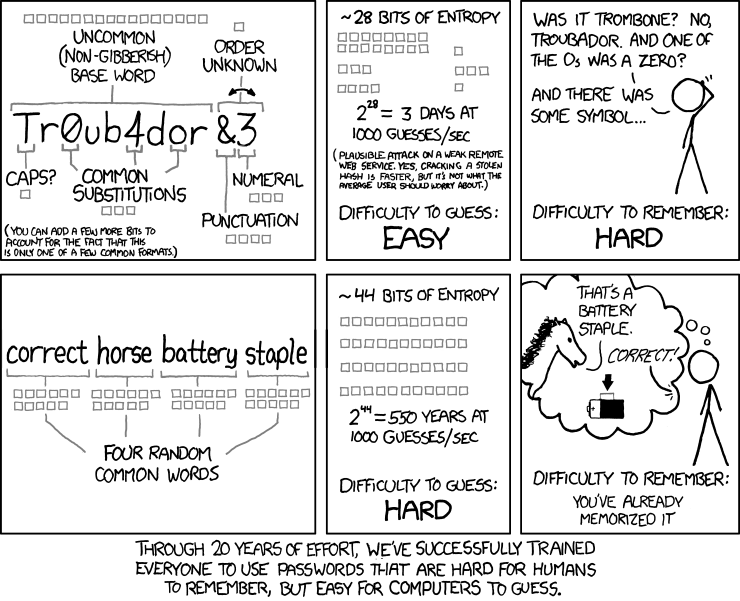
\includegraphics[width=\linewidth]{./images/password_strength.png}
\caption[Recommandations pour un mot de passe fort, par XKCD (https://xkcd.com/936/)]{}
\end{figure}

\emph{Bonus pour les profs de français ou les gens vivants en pays
étranger} :\\utilisez un mot compliqué, tel qu'un verbe particulièrement
ardu de la langue française à un temps de conjugaison improbable, et
hop, le mot de passe est presque impossible à trouver pour un humain
puisque peu de monde comprend votre langue, du moins à ce niveau.

Moi, ce que je fais, c'est que je prends un ou des mots de mon
environnement immédiat, ou un concept auquel je pense (en français, donc
j'ai déjà l'avantage indiqué au dessus).\\Puis je le \emph{tords}. Je
remplace le A par un À ou un @. Le L par ! ou autre chose du même genre.
J'ajoute des chiffres à un endroit choisi dans le mot.

Deux ou trois changements de cet acabit et le mot est méconnaissable et
donc difficile à deviner pour un humain, et un ordinateur (à cause de sa
longueur).

\subsubsection{De l'utilité de la passhprase}\label{de-lutilituxe9-de-la-passhprase}

Vous pouvez choisir de ne pas mettre de passhprase. Je dois avouer ne
pas l'avoir fait durant un long moment. Aujourd'hui je le fais et je le
recommande.

Ça ajoute tout simplement une sécurité supplémentaire. Chaque fois que
vous utiliserez votre clé, pour signer ou déchiffrer un message, ce mot
de passe vous sera demandé.\\Si vous n'êtes pas le seul à utiliser votre
ordinateur, ou si vous utilisez vos clés gpg sur votre tablette ou votre
smartphone (qu'on laisse fréquemment accessible sans le verrouiller),
alors vous avez intérêt à donner une passhprase.

\subsubsection{Certificat de revocation}\label{certificat-de-revocation}

Il est très probable que le gestionnaire de clé vous propose de générer
un certificat de révocation. C'est en effet une très bonne chose, donc
faîtes le s'il vous plait.

En cas de perte de la clé, de corruption, que quelqu'un entre en
possession de votre clé privée, hop, on publie ce certificat de
révocation sur les serveurs de clés. Très rapidement, par le jeu des
mises à jour mutuelles des serveurs, la clé est marquée comme invalide
sur l'ensemble du monde internet.

Ceci constitue donc une sécurité pour le cas où on vous volerait la clé
privée.

\emph{Si le logiciel ne vous propose pas la création d'un certificat de
révocation, ne vous en faîtes pas, je vous expliquerais la démarche en
détail dans un article futur.}

Si vous voulez changer de clé proprement, ce n'est absolument pas la
bonne méthode. Je vous en parlerais dans un autre article.

\section{Exercice}\label{exercice}

Comme j'ai pensé ce tutoriel comme pédagogique, je vais faire des petits
exercices ici et dans les articles suivants. Pour les besoins de ces
exercices, j'ai créée une adresse courriel sur mon serveur et des clés
pour cette adresse.

\textbf{\emph{Ces clés ne seront jamais utilisées pour une autre raison
que ce tutoriel.}}

Je vais vous demander en l'occurence d'exporter votre clé publique
fraichement générée, et de me l'envoyer en courriel, tout simplement.
C'est ce que beaucoup de personnes font pour échanger leurs clés.

Je vous renverrais alors un courriel où je vous dirais si votre clé a
les bonnes caractéristiques. J'ai également besoin de votre clé pour
l'exercice de l'article suivant.

\subsection{Exporter sa clé}\label{exporter-sa-cluxe9}

Pour m'envoyer votre clé, il vous faut l'\emph{exporter}.

Pour se faire, vous devez le demander à votre gestionnaire de clés.

Faîtes bien attention, votre gestionnaire de clés pourra vous proposer
d'exporter la paire de clés complète ou la clé privée.

Je parle bien, ici, de votre clé \textbf{publique} !

En effet, comme on l'a déjà signalé plus tot, et comme son nom l'indique
bien, la clé publique est à la disposition de tous.\\Le gestionnaire de
clé va vous proposer l'exportation de votre clé sous forme d'un fichier
d'extension gpg ou asc.

Ce fichier est en fait un bête fichier texte, qui contient la clé
publique, sous la forme d'une longue suite de caractères. Vous pouvez en
effet ouvrir le fichier avec Notepad ou un autre éditeur de texte par
exemple.

\emph{Et non, OpenOffice ou Word ne sont pas des éditeurs texte!}

\textbf{\emph{Toutefois, si vous ouvrez le fichier texte, ne le modifiez
surtout pas !}}

Vous pouvez alors me l'envoyer en pièce jointe d'un courriel à
\emph{Tuto-gpg @ 22decembre.eu}. Ni plus, ni moins.

\emph{NB : Kmail (client courriel de KDE), propose également dans son menu }\textbf{Joindre\ldots{}}* de mettre sa clé publique en pièce
jointe du courriel. Tout simple.